\scanpage{17}
\mspage{6}

de spécialisation $D\mathbin{-}D'$ définit une flèche $\operatorname{Gen}_0(D)\hookrightarrow\operatorname{Gen}_0(D')$ injective, dont le complémentaire est formé de deux \deleted{sommets} éléments \deleted{$\unsure{a}$}.

\deleted{\unsure{Immersion}}\inserted{Plongement} cellulaire canonique de $\Gamma(\underline\Sigma)$ dans une surface \deleted{\unsure{combinatoire}}\inserted{$\operatorname{Str}(\underline\Sigma)$ (la surface structurale)}

Sommets stables: toutes les arêtes qui en sortent \uline{partent} de $D$
\figure{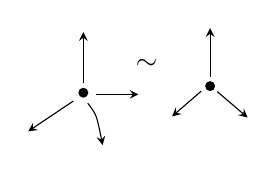
\begin{tikzpicture}[x=.7cm,y=.7cm,>=stealth]
\fill (0,0) circle(1.8pt);\draw[->] (0,.18)--(0,1.1);\draw[->] (-.18,-.15)--(-1,-.70);\draw[->] (.08,-.19)..controls(.24,-.4)..(.35,-.95);\draw[->] (.23,-.03)--(1,-.03);
\node at (1.15,.52){$\sim$};
\fill (2.3,.12) circle(1.8pt);\draw[->] (2.3,.28)--(2.3,1.17);\draw[->] (2.14,.03)--(1.61,-.43);\draw[->] (2.43,.02)--(2.98,-.45);
\end{tikzpicture}}

Sommets sous-stables: il y a exactt \uline{deux} arêtes qui \uline{arrivent} à $D$
\figure{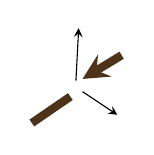
\begin{tikzpicture}[x=.7cm,y=.7cm,>=stealth]
\draw[->] (0,.17)--(.05,1.12);\draw[->] (.12,-.03)--(.75,-.45);
\draw[->,brown!40!black,line width=3pt] (-.8,-.60)--(-.1,-.12) (.83,.63)--(.12,.20);
\end{tikzpicture}}

Sommets critiques: au moins quatre arêtes qui arrivent à $D$
\figure{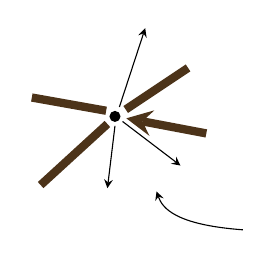
\begin{tikzpicture}[x=.8cm,y=.8cm,>=stealth]
\fill (0,0) circle(2pt);\draw[->] (.07,.15)--(.48,1.4);\draw[->] (0,-.15)--(-.12,-1.14);\draw[->] (.12,-.08)--(1.04,-.78);
\draw[->,brown!40!black,line width=3pt] (-1.32,.30)--(-.14,.09) (-1.18,-1.09)--(-.12,-.12) (1.16,.77)--(.17,.11) (1.45,-.27)--(.18,-.03);
\draw[->] (2.03,-1.80).. controls(.95,-1.72) and (.75,-1.45)..(.66,-1.19);
\end{tikzpicture}}

Sommets critiques \deleted{\unsure{et}} extrémaux: toutes les arêtes en $D$ \uline{arrivent} à $D$
\figure{
\begin{tikzpicture}[x=.7cm,y=.7cm,>=stealth]
\fill (0,0) circle(2pt);\draw[->,brown!40!black,line width=3pt] (-.85,.85)--(-.12,.11) (.77,.86)--(.11,.12) (-.81,-.92)--(-.10,-.12) (.81,-.88)--(.12,-.13);
\end{tikzpicture}}

\uline{Toute arête} de $\Gamma(\underline\Sigma)$ est munie d'un \uline{poids} $(\in\mathbf N^*)$ qui \inserted{est le} \deleted{\unsure{pour une arête de spécialisation}} \deleted{\unsure{également exprimé}} \inserted{\unsure{nb d'arêtes}} \deleted{de} $D$ (ou resp. de $\Sigma'$, interceptées par l'arc de spécialisation) --- dans le cas de la figure ci-contre, correspondant au triangle de spécialisation $T$.

\figure{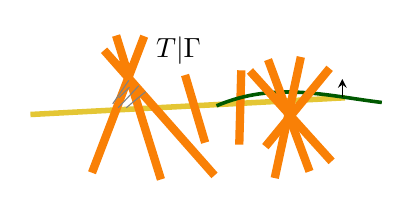
\begin{tikzpicture}[x=.85cm,y=.85cm,>=stealth]
\draw[yellow!55!brown,line width=2pt] (-1.6,-.05)--(3.1,.20);
\draw[orange!90!brown,line width=3pt] (-.68,-.92)--(.1,1.12) (-.32,1.13)--(.35,-1.02) (-.50,.91)--(1.15,-.96) (.71,.54)--(1.01,-.47) (1.55,.61)--(1.52,-.50);
\draw[gray,thin] (-.28,.20)--(-.12,.36) (-.37,.11)--(-.13,.46) (-.29,.05)--(.02,.38) (-.17,.05)--(.12,.29);
\node[above right] at (.13,.55){$\unsure{T|\Gamma}$};
\draw[green!35!black,line width=1.3pt] (1.18,.08)..controls(2.05,.45) and (2.82,.23)..(3.65,.13);
\foreach \a/\b/\c/\d in {1.68/.60/2.90/-.75,1.95/.77/2.57/-.90,2.44/.81/2.05/-1.0,2.87/.64/1.91/-.53}{\draw[orange!90!brown,line width=3pt](\a,\b)--(\c,\d);}
\draw[->] (3.06,.21)--(3.06,.48);
\end{tikzpicture}}

Tout secteur cellulaire local de $\operatorname{Str}(\underline\Sigma)$ en un sommet $D$ correspond à un arc de $\widetilde D$, \deleted{correspondant à l'arc}\inserted{simple} \uline{l'arc} compris entre deux arcs de spécialisation consécutifs, ou deux \deleted{arcs de} sommets de \deleted{spécialisation}\inserted{générisation} consécutifs (sur $\widetilde D$, sans aucun arc de spécialisation entre), ou les cas mixtes; le nb d'arêtes sur cet arc (au sens de $\Sigma'$) est appelé encore \uline{poids} du secteur angulaire. Avec ces données, on trouve une \uline{carte cellulaire} \deleted{pondérée} \uline{à graphe orienté}, et à arêtes et ``coins'' \uline{pondérés}. On a d'autre part, pour tt sommet $D$,

\margin{\deleted{\unsure{de toutes les}} somme des \inserted{pondérations de} toutes les arêtes en $D$, et des \inserted{pondérations de} tous les coins en $D$ \deleted{$\unsure{\longleftarrow}$} est égale à $2n$ (où $n=\operatorname{card}\Sigma$)}
\margin{16}
